% !TEX root =../main.tex

\chapter{Auswahl an Konzepten Festlegen}


\section{Voraussetzung bei der Entwicklung}


% TODO: Was bedeutet die Viskosität zwichen Nutzer und Webseite?
\subsection{Viskosität zwischen Nutzer und die Webseite verstärken}

% TODO: Vollständigen Namen des Institus Nielsen angeben. Vielleicht als Fußnote.
% TODO: Genaues Datum angeben bei `Nielsens am Dienstag veröffentlichte ...'
% TODO: Bitte wörtliches Zitat auf Korrektheit überprüfen: `ist drei Viertel der Online-Nutzer auf der Welt zugreifen können.'
% TODO: Genauen Zeitraum angeben bei `haben im vergangenen Monat ...'. Besser ist `haben im Mail 2018 ...'.

Laut dem Marktforschungsunternehmen Nielsen verbringen Nutzer mit Instant Messaging, dem Schreiben von Kommentaren, Bloggen, Teilen und \glqq{}Liken\grqq{} durchschnittlich 22\% ihrer Online-Zeit. Nielsens am Dienstag veröffentlichte Statistik zeigte, dass Menschen alle 4,5 Minuten ihrer Online-Zeit eine Minute in sozialen Netzwerken verbringen. Internetnutzer verbringen somit jeden Monat 110 Milliarden Minuten in sozialen Netzwerken und Blogs. Die Umfrage sagt, dass dies dass erste Mal ist, dass ein soziales Netzwerk oder ein Blog \glqq{}ist drei Viertel der Online-Nutzer auf der Welt zugreifen können.\grqq{} Das ist eine Steigerung von 24\% gegenüber dem gleichen Zeitraum des Vorjahres. Die beliebtesten Social-Networking-Marken sind Facebook und YouTube. Online-Nutzer haben im vergangenen Monat 13 Milliarden Videos auf YouTube gesehen. Facebook meldete, dass seine Nutzer 2 Milliarden Videos pro Monat sehen.

% TODO: (Nielsen-Studie: Facebook und Google haben erfolgreichste Apps Jonas Wagner) in litertur.bib einfügen. `

Laut Nielsens Studie hat Facebook in den globalen Online-Stunden das Rampenlicht übernommen. Fast 500 Millionen Nutzer verbringen jeden Monat sechs Stunden damit.
Was die Netzabdeckung betrifft, übernimmt Google die Führung. Laut Nielsen-Statistiken besuchen 82\% der Internetnutzer weltweit jeden Monat diese Website, und die durchschnittliche Suchzeit beträgt 1 Minute und 20 Sekunden.(Nielsen-Studie: Facebook und Google haben erfolgreichste Apps Jonas Wagner)

D.h. die Länge der Zeit, welche ein Nutzer auf einer Webseite verbringt, ist ein Zeichen dafür, ob diese Webseite beliebt ist und ob die Viskosität stark ist.

Ein wichtige Frage bei dem Entwurf einer Webseite ist, wie man Nutzer motiviert, mehr Zeit auf dieser Webseite zu verbringen. Durch interessante Funktionen und Veranstaltungen?


\subsection{Online Shops welche mehr Produkte verkaufen sind beliebter}

Nach der Statistik von Alexa in Abbildung \vref{fig:alexa}, sind die Top 10 Webshops mit dem höchsten Umsatz unter anderem Amazon, Netflix, Ebay, Walmart, Etsy, Steam und Ikea. Sie alle haben eine Gesamtheit: Es ist eine hohe Vielfalt an Produkten verfügbar.

\begin{figure}
	\centering
	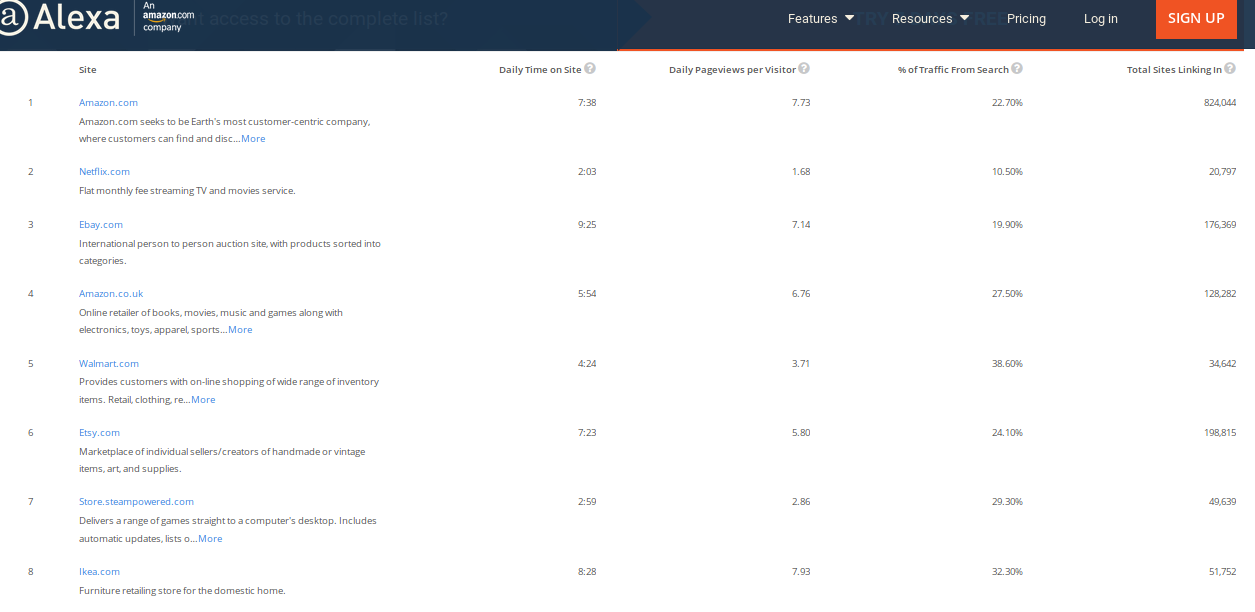
\includegraphics[width=1\textwidth]{bilder/alexa.png}
	\caption{Alexa}
	\label{fig:alexa}
\end{figure}


\section{Freunde organisieren}

Man verwendet Listen, um  Freunde organisieren. Mit einer Liste kann man die Meldungen in seinem News-Feed filtern oder Aktualisierungen mit bestimmten Personen teilen. Z. B. mit Arbeitskollegen oder Freunden, die in der Nähe wohnen. Man kann jederzeit Freunde hinzufügen order entfernen. \parencite{facebook:help}

\textbf{Enge Freunde:} Freunde, mit denen man möglicherweise alles teilen möchte.

\textbf{Bekannte:} Personen, mit denen man eventuell weniger teilen möchte.

\textbf{Eingeschränkt:} Diese Liste ist für Personen, die man als Freunde hinzugefügt hat, mit denen man aber nichts teilen möchte. Z. B. einem Arbeitskollegen oder Vorgesetzten.

Man kann außerdem selbst definierte Listen erstellen,  um selbst Freunde in Gruppen zusammenzufassen. Der Nutzer legst fest, wer zu einer bestimmten Liste hinzugefügt wird und welche Privatsphäre-Einstellungen (gegebenenfalls) gelten. Es ist zu beachten, dass Freunde nicht benachrichtigt werden, wenn sie zu benutzerdefinierten Liste hinzufügt werden.


\section{Echtzeitkommunikation mit anderen Nutzern, Verkäufern und dem Kundenservice der Plattform}

Ein potentieller Nachteil von Amazon ist, dass es schwer ist mit dem Verkäufer oder dem Kundenservice persönlich in Kontakt zu treten. Dadurch kann das Kommunizieren und Lösen von Problemen zeitaufwändig und kompliziert ausfallen.

Durch die Verwendung von Echtzeit-Kommunikation, können Probleme unter Umständen deutlich schneller und unkomplizierter gelöst werden. Dies könnte das Einkaufserlebnis deutlich verbessern.


\section{Offline Kontakte}

Gleichzeit eine URL als Nachricht per E-Mail und SMS versenden, welche die Produktinformation beinhaltet. Freunde oder Bekannte müssen sich so nicht noch einmal anmelden, sonder können direkt die URL anklicken. Dadurch werden sie automatisch in die Bestehende Sitzung des Käufern eingeloggt und können sofort Vorschläge unterbreiten und bei der Entscheidungsfindung unterstützen.


\section{Nach dem Handel, Erfahrung und Bewertung teilen und Produkt mit Freunden teilen}


\section{Pay by others}

Wenn ein Kind die finanzielle Hilfe der Eltern benötigt, können sich die Eltern auch in dem genutzten Webshop einloggen und entscheiden, ob sie für die Produkte des Kindes bezahlen wollen.


\section{Zusätzliche Services}


\subsection{Weitere Entwicklungen auf der Basis von Ebay Kleinanzeigen}

Von Ebay Kleinanzeigen zum online Flohmarkt.

Gebrauchte Produkte werden auf der Webseite angezeigt. Die Produkte werden nicht mehr nach einzelnen Attributen klassifiziert, sondern werden gemäß ihrem Verkäufer gruppiert. Ähnlich wie bei dem Besuch eines Flohmarktes. Die gebrauchten Produkte werden nicht nach Attributen sortiert aufgestellt. Z.B. werden nicht alle Spielzeuge des Flohmarkts an einer Stelle verkauft, sonder die Produkte sind nach ihrer Quelle, ihrem Verkäufer sortiert.


\subsection{Communities  für die Nutzer erstellen, um Nachrichten zu veröffentlichen und Erfahrung auszutauschen}

\begin{itemize}
\item Kooperation existiert vor allem in Computerspielen
\item Darstellung und Interaktion im Webshop wird denen von Computerspielen nachempfunden
\item 3D Darstellung und Steuerung wie in Computerspielen
\end{itemize}